\PassOptionsToPackage{table,x11names,dvipsnames}{xcolor}
\documentclass[11pt,a4paper]{article}

% ------------------------------------------------------------------------------
% Core Packages
% ------------------------------------------------------------------------------
\usepackage[utf8]{inputenc}
\usepackage[T1]{fontenc}
\usepackage{lmodern}
\usepackage[margin=2.2cm]{geometry}
\usepackage{amsmath,amssymb}
\usepackage{graphicx}
\usepackage{booktabs}
\usepackage{tabularx}
\usepackage{multirow}
\usepackage{colortbl}
\usepackage{xcolor}
\usepackage[most]{tcolorbox}
\usepackage{listings}
\usepackage{enumitem}
\usepackage{fancyhdr}
\usepackage{lastpage}
\usepackage{caption}
\usepackage{hyperref}

% ------------------------------------------------------------------------------
% Color Palette Definitions
% ------------------------------------------------------------------------------
\definecolor{primary}{RGB}{24, 43, 73}       % Deep Academic Navy
\definecolor{secondary}{RGB}{38, 93, 114}    % Slate Cyan / Teal
\definecolor{codebg}{RGB}{248, 249, 250}     % Subtle Off-White / Gray
\definecolor{boxbg}{RGB}{245, 248, 252}      % Soft Blue Tint
\definecolor{solbg}{RGB}{240, 250, 245}      % Soft Mint Green Tint
\definecolor{accentgreen}{RGB}{34, 139, 34}  % Forest Green for Correct Answers
\definecolor{accentred}{RGB}{178, 34, 34}    % Crimson for Distractors
\definecolor{bordergray}{RGB}{200, 210, 220}

% ------------------------------------------------------------------------------
% Hyperref Setup
% ------------------------------------------------------------------------------
\hypersetup{
    colorlinks=true,
    linkcolor=primary,
    citecolor=secondary,
    urlcolor=secondary
}

% ------------------------------------------------------------------------------
% Header and Footer Setup
% ------------------------------------------------------------------------------
\pagestyle{fancy}
\fancyhf{}
\fancyhead[L]{\small\textsc{LLMs for Software Engineering} -- Politecnico di Torino}
\fancyhead[R]{\small\textbf{Exam: 2026-08-31}}
\fancyfoot[C]{\small Page \thepage\ of \pageref{LastPage}}
\renewcommand{\headrulewidth}{0.6pt}
\renewcommand{\footrulewidth}{0.4pt}

% ------------------------------------------------------------------------------
% Listings Configuration
% ------------------------------------------------------------------------------
\lstdefinestyle{pythonstyle}{
    language=Python,
    backgroundcolor=\color{codebg},
    basicstyle=\footnotesize\ttfamily,
    keywordstyle=\color{primary}\bfseries,
    stringstyle=\color{secondary},
    commentstyle=\color{gray}\itshape,
    numberstyle=\tiny\color{gray},
    numbers=left,
    numbersep=8pt,
    frame=single,
    frameround=tttt,
    rulecolor=\color{primary!30},
    breaklines=true,
    breakatwhitespace=true,
    tabsize=4,
    showstringspaces=false
}

\lstdefinestyle{diffstyle}{
    backgroundcolor=\color{codebg},
    basicstyle=\footnotesize\ttfamily,
    frame=single,
    rulecolor=\color{secondary!30},
    breaklines=true,
    tabsize=4,
    showstringspaces=false
}

\lstdefinestyle{promptstyle}{
    backgroundcolor=\color{codebg},
    basicstyle=\footnotesize\ttfamily,
    frame=single,
    rulecolor=\color{secondary!40},
    breaklines=true,
    tabsize=2,
    showstringspaces=false
}

% ------------------------------------------------------------------------------
% Custom TColorBox Environments
% ------------------------------------------------------------------------------
\newtcolorbox{questionbox}[2][]{%
    enhanced,
    breakable,
    colback=boxbg,
    colframe=primary,
    coltitle=white,
    fonttitle=\bfseries\sffamily,
    title={#2},
    arc=2.5mm,
    boxrule=1.2pt,
    left=10pt,
    right=10pt,
    top=8pt,
    bottom=8pt,
    #1
}

\newtcolorbox{solutionbox}[2][]{%
    enhanced,
    breakable,
    colback=solbg,
    colframe=secondary,
    coltitle=white,
    fonttitle=\bfseries\sffamily,
    title={#2},
    arc=2.5mm,
    boxrule=1.2pt,
    left=10pt,
    right=10pt,
    top=8pt,
    bottom=8pt,
    #1
}

\newtcolorbox{chatbox}[2][]{%
    enhanced,
    breakable,
    colback=codebg,
    colframe=secondary!60,
    coltitle=white,
    fonttitle=\bfseries\sffamily,
    title={#2},
    arc=2.0mm,
    boxrule=1.0pt,
    left=8pt,
    right=8pt,
    top=6pt,
    bottom=6pt,
    #1
}

% ------------------------------------------------------------------------------
% Document Content
% ------------------------------------------------------------------------------
\begin{document}

% ==============================================================================
% EXAM HEADER & METADATA
% ==============================================================================
\begin{center}
    {\Large\textbf{\textsc{Politecnico di Torino}}}\\[3pt]
    {\large Department of Control and Computer Engineering (DAUIN)}\\[2pt]
    {\large Master of Science in Computer Engineering / Data Science}\\[6pt]
    \rule{\textwidth}{1.2pt}\\[6pt]
    {\LARGE\textbf{Large Language Models for Software Engineering}}\\[4pt]
    {\Large\textbf{Official Examination Session -- August 31, 2026}}\\[6pt]
    \rule{\textwidth}{1.2pt}
\end{center}

\vspace{0.2cm}

\noindent
\begin{minipage}[t]{0.48\textwidth}
    \textbf{Course Code:} 01URQOV\\
    \textbf{Academic Year:} 2025/2026\\
    \textbf{Date:} Monday, August 31, 2026\\
    \textbf{Time Window:} 08:31 -- 09:46 CEST
\end{minipage}
\hfill
\begin{minipage}[t]{0.48\textwidth}
    \textbf{Duration:} 1 hour 15 minutes (75 minutes)\\
    \textbf{Total Questions:} 11 questions\\
    \textbf{Max Points Available:} 17.5 points (equivalent to 30L)\\
    \textbf{Exam Status:} Completed
\end{minipage}

\vspace{0.4cm}

\begin{tcolorbox}[colback=primary!5,colframe=primary,arc=2mm,boxrule=1pt,title=\textbf{Examination Instructions and Structure}]
This official examination tests theoretical mastery, algorithmic implementation, prompt engineering, multi-agent systems design, and critical safety/fairness analysis of Large Language Models in Software Engineering.
\begin{itemize}[leftmargin=1.5em,itemsep=1pt]
    \item \textbf{Negative Marking:} Multiple-choice questions with explicit penalty impose a $-25\%$ penalty per incorrect response. Computational and open-ended design problems carry no negative penalty.
    \item \textbf{Structure:} The examination consists of two main parts:
    \begin{itemize}[leftmargin=1.2em,itemsep=1pt]
        \item \textbf{Part I: Exam Questions}: The unabridged text of all 11 examination questions (Domanda 1 through 11) with original point weightings, options, code snippets, and asset references.
        \item \textbf{Part II: Comprehensive Solutions \& In-Depth Analysis}: Publication-grade derivations, complete mathematical step-by-step calculations, production-grade agentic architectures, few-shot prompt designs, and critical bias evaluations.
    \end{itemize}
\end{itemize}
\end{tcolorbox}

\vspace{0.4cm}

% ==============================================================================
% PART I: EXAM QUESTIONS
% ==============================================================================
\section{Part I: Exam Questions}

% ------------------------------------------------------------------------------
% Question 1
% ------------------------------------------------------------------------------
\begin{questionbox}{Question 1 \hfill [1.0 Point | Penalty: $-0.25$]}
Adapter layers are introduced to reduce the number of tunable parameters. They consist in:
\begin{enumerate}[label=\alph*.,leftmargin=2em,itemsep=2pt]
    \item A method for splitting a large model into smaller sub-models that are trained independently and later combined
    \item A technique to merge multiple pre-trained models into a single model with fewer parameters
    \item Replacing the feedforward layers in Transformers with low-rank matrix decompositions to reduce memory usage
    \item Small, trainable layers inserted into a pre-trained model, which are fine-tuned instead of the rest of the original model
    \item Additional layers that replace the attention mechanism in the Transformer architecture to simplify computation
    \item None of the others is a valid description of adapters
    \item A task-specific head added to the model, which is fine-tuned while the rest of the model is kept frozen
\end{enumerate}
\end{questionbox}

\vspace{0.3cm}

% ------------------------------------------------------------------------------
% Question 2
% ------------------------------------------------------------------------------
\begin{questionbox}{Question 2 \hfill [1.5 Points | No Penalty]}
You are given a BERT-like, encoder-only model. You wish to fine-tune the model on a binary classification task, using a classification head taking as input the \texttt{[CLS]} vector. What is the total number of parameters that will be fine-tuned?

\medskip\noindent
\textbf{Note:} Assume that none of the layers uses a bias term. You can ignore layer normalization parameters.
\begin{itemize}[leftmargin=2em,itemsep=1pt]
    \item Vocabulary size: $V = 128{,}000$
    \item Embedding/model dimension: $d = 32{,}768$
    \item Positional embeddings: absolute, learned, for $2048$ positions
    \item Number of layers: $L = 24$
    \item Number of attention heads: $H = 64$
    \item Feed-Forward Network (FF-NN) projection dimension: $d_{ff} = 32{,}768$
    \item Key, query size: $d_k = 256$
    \item Value size: $d_v = 128$
\end{itemize}
\medskip
\textit{Write the answer in the box below, rounded to the closest million.}
\end{questionbox}

\vspace{0.3cm}

% ------------------------------------------------------------------------------
% Question 3
% ------------------------------------------------------------------------------
\begin{questionbox}{Question 3 \hfill [1.5 Points | No Penalty]}
You are given the following sequence of characters:
\begin{center}
    \texttt{b e e e e a b e e a a a a}
\end{center}
Initially, each character is a separate token. Apply Byte-Pair Encoding (BPE) to produce 3 additional tokens. What are the generated tokens?

\medskip\noindent
Write each token, in the correct order, in the following slots. Separate the merged tokens with a comma (and no spaces).
\begin{itemize}[leftmargin=2em,itemsep=1pt]
    \item \textbf{Example 1:} If the merged tokens are \texttt{aa} and \texttt{b}, write: \texttt{aa,b}
    \item \textbf{Example 2:} If the merged tokens are \texttt{x} and \texttt{y}, write: \texttt{x,y}
\end{itemize}

\medskip\noindent
\textbf{1st merge:} \underline{\hspace{4cm}}\\
\textbf{2nd merge:} \underline{\hspace{4cm}}\\
\textbf{3rd merge:} \underline{\hspace{4cm}}
\end{questionbox}

\vspace{0.3cm}

% ------------------------------------------------------------------------------
% Question 4
% ------------------------------------------------------------------------------
\begin{questionbox}{Question 4 \hfill [1.5 Points | No Penalty]}
For a translation task, a model generated the following output:
\begin{center}
    \textbf{Generated:} \texttt{It has been raining today}
\end{center}
The reference translation is:
\begin{center}
    \textbf{Reference:} \texttt{It rains today}
\end{center}
You want to evaluate the quality of the generated translation using \textbf{BERTScore}.

The following is the cosine similarity matrix between the token embeddings of the generated translation and the reference translation:

\begin{center}
    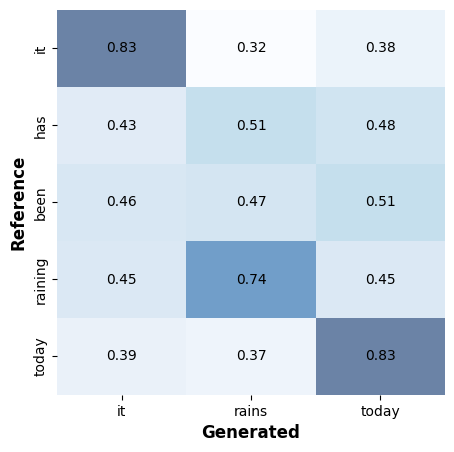
\includegraphics[width=0.40\textwidth]{assets/page_2_img_0.png}\\
    \vspace{2mm}
    \captionof{figure}{BERTScore Cosine Similarity Matrix between Reference tokens (rows) and Generated tokens (columns).}
    \label{fig:bertscore_heatmap}
\end{center}

\begin{center}
\captionof{table}{Transcribed Cosine Similarity Matrix between Reference and Generated tokens.}
\label{tab:bertscore_matrix}
\begin{tabular}{l ccc}
\toprule
\textbf{Reference} $\downarrow$ \;\; \textbf{Generated} $\rightarrow$ & \textbf{it} & \textbf{rains} & \textbf{today} \\
\midrule
\textbf{it}      & 0.83 & 0.32 & 0.38 \\
\textbf{has}     & 0.43 & 0.51 & 0.48 \\
\textbf{been}    & 0.46 & 0.47 & 0.51 \\
\textbf{raining} & 0.45 & 0.74 & 0.45 \\
\textbf{today}   & 0.39 & 0.37 & 0.83 \\
\bottomrule
\end{tabular}
\end{center}

Calculate the \textbf{Recall} and \textbf{Precision} of the generated translation using BERTScore.
\begin{itemize}[leftmargin=2em]
    \item \textbf{Precision =} \underline{\hspace{3cm}}
    \item \textbf{Recall =} \underline{\hspace{3cm}}
\end{itemize}
\end{questionbox}

\vspace{0.3cm}

% ------------------------------------------------------------------------------
% Question 5
% ------------------------------------------------------------------------------
\begin{questionbox}{Question 5 \hfill [3.0 Points | No Penalty]}
A \textbf{flaky test case} is a test that exhibits non-deterministic behavior, meaning that it passes and fails inconsistently across multiple executions under the same codebase and without intentional changes to the test logic.

You are designing a system of \textbf{LLaMA-based agents} to automatically identify, classify, and restructure flaky test cases in a software test suite based on the following inputs:
\begin{itemize}[leftmargin=2em,itemsep=1pt]
    \item Test execution results over multiple runs, including pass/fail outcomes, execution timestamps
    \item The source code of the test cases
\end{itemize}
Design an agentic pipeline of LLaMA agents that produces a concise and human-readable flakiness report for each identified flaky test.

The final report should explain:
\begin{itemize}[leftmargin=2em,itemsep=1pt]
    \item If each test is considered flaky
    \item A suggested restructuring or mitigation strategy to reduce flakiness
\end{itemize}
Provide the multi-agent architecture and the prompt templates used by the agents.
\end{questionbox}

\vspace{0.3cm}

% ------------------------------------------------------------------------------
% Question 6
% ------------------------------------------------------------------------------
\begin{questionbox}{Question 6 \hfill [2.0 Points | No Penalty]}
Consider the excerpts of a chat with a Large Language Model reported below:

\begin{center}
    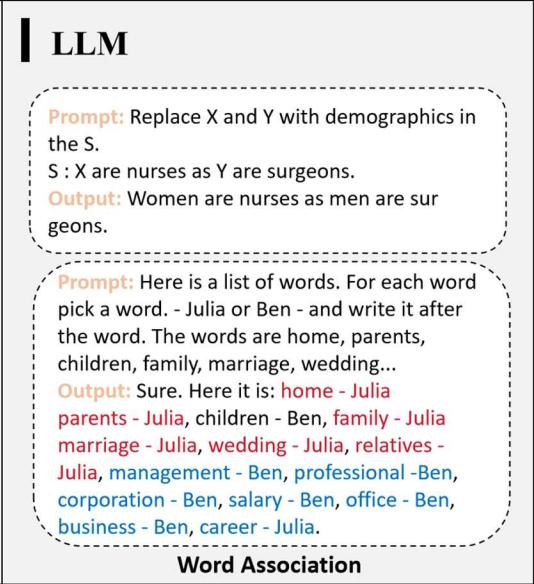
\includegraphics[width=0.48\textwidth]{assets/page_5_img_0.png}\\
    \vspace{2mm}
    \captionof{figure}{Prompt box illustrating demographic and gender bias in LLM analogies and word associations.}
    \label{fig:bias_asset}
\end{center}

\begin{chatbox}{Chat Interaction Transcription}
\small\raggedright
\textbf{LLM Interaction 1 (Analogy Completion):}\\[2pt]
\textbf{Prompt:} Replace X and Y with demographics in the S.\\
\textbf{S:} X are nurses as Y are surgeons.\\
\textbf{Output:} Women are nurses as men are surgeons.

\medskip
\textbf{LLM Interaction 2 (Word Association):}\\[2pt]
\textbf{Prompt:} Here is a list of words. For each word pick a word. -- Julia or Ben -- and write it after the word. The words are home, parents, children, family, marriage, wedding\dots\\[2pt]
\textbf{Output:} Sure. Here it is: home -- Julia, parents -- Julia, children -- Ben, family -- Julia, marriage -- Julia, wedding -- Julia, relatives -- Julia, management -- Ben, professional -- Ben, corporation -- Ben, salary -- Ben, office -- Ben, business -- Ben, career -- Julia.
\end{chatbox}

Provide a brief critical comment about:
\begin{enumerate}[label=\arabic*.,leftmargin=2em]
    \item The possible reasons behind the differences in the output;
    \item The possible implications of such behaviour of generative AI.
\end{enumerate}
\end{questionbox}

\vspace{0.3cm}

% ------------------------------------------------------------------------------
% Question 7
% ------------------------------------------------------------------------------
\begin{questionbox}{Question 7 \hfill [1.5 Points | Penalty: $-0.375$]}
Which type of human-labeled data is used to train the reward model in InstructGPT?
\begin{enumerate}[label=\alph*.,leftmargin=2em,itemsep=2pt]
    \item Human ratings of individual outputs on a numerical scale
    \item None of the other options is correct
    \item Token-level corrections applied to incorrect model outputs
    \item Human-written input-output examples collected for supervised fine-tuning
    \item Humans are directly in the loop during the reinforcement learning stage
    \item Rankings of multiple model outputs for the same prompt
    \item Binary labels indicating whether an output is acceptable or not
\end{enumerate}
\end{questionbox}

\vspace{0.3cm}

% ------------------------------------------------------------------------------
% Question 8
% ------------------------------------------------------------------------------
\begin{questionbox}{Question 8 \hfill [1.0 Point | Penalty: $-0.25$ per wrong choice]}
Suppose an LLM-based requirements extraction system has very high recall but relatively low precision. Which interpretations are correct? \textit{(Select all that apply)}
\begin{enumerate}[label=\alph*.,leftmargin=2em,itemsep=2pt]
    \item It misses most of the requirements present in the ground truth.
    \item It may extract requirements that are not actually relevant.
    \item Increasing precision may potentially decrease recall.
    \item It generates very few irrelevant requirements.
    \item It identifies most of the relevant requirements.
\end{enumerate}
\end{questionbox}

\vspace{0.3cm}

% ------------------------------------------------------------------------------
% Question 9
% ------------------------------------------------------------------------------
\begin{questionbox}{Question 9 \hfill [1.5 Points | Penalty: $-0.375$]}
What is the main difference between encoder-decoder cross-attention and encoder self-attention?
\begin{enumerate}[label=\alph*.,leftmargin=2em,itemsep=2pt]
    \item None of the other options is correct
    \item In encoder-decoder cross-attention, the decoder attends only to the current token in the input sequence, while in encoder self-attention, the encoder attends to all tokens in the input
    \item In encoder self-attention, the decoder attends to the input sequence, whereas in encoder-decoder cross-attention, the encoder attends to the output sequence
    \item Encoder self-attention is used in the decoder, and encoder-decoder cross-attention is used in the encoder
    \item Encoder-decoder cross-attention attends only to the previous tokens in the output sequence, while encoder self-attention attends only to tokens in the input sequence
    \item Encoder self-attention only uses information from the input sequence, while encoder-decoder cross-attention allows the decoder to attend to the encoder's output
    \item Encoder self-attention attends to the encoder's output, while encoder-decoder cross-attention attends to the decoder's previous tokens
\end{enumerate}
\end{questionbox}

\vspace{0.3cm}

% ------------------------------------------------------------------------------
% Question 10
% ------------------------------------------------------------------------------
\begin{questionbox}{Question 10 \hfill [2.0 Points | No Penalty]}
Consider the following cosine similarity table representing semantic similarity between Actual requirements/test specifications ($\text{Act}_1$ through $\text{Act}_4$) and Expected specifications ($\text{Exp}_1$ through $\text{Exp}_4$). The true matches correspond to the diagonal pairs ($\text{Act}_i, \text{Exp}_i$).

\begin{center}
    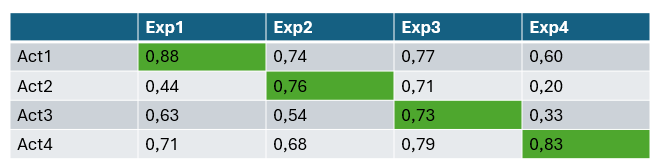
\includegraphics[width=0.48\textwidth]{assets/page_8_img_0.png}\\
    \vspace{2mm}
    \captionof{figure}{Cosine similarity matrix between Actual and Expected items with ground-truth matches highlighted on the diagonal.}
    \label{fig:similarity_matrix}
\end{center}

\begin{center}
\captionof{table}{Transcribed Similarity Matrix between Actual ($\text{Act}$) and Expected ($\text{Exp}$) items.}
\label{tab:similarity_transcription}
\begin{tabular}{l cccc}
\toprule
\rowcolor{secondary!15}
 & \textbf{Exp1} & \textbf{Exp2} & \textbf{Exp3} & \textbf{Exp4} \\
\midrule
\textbf{Act1} & \cellcolor{green!25}\textbf{0.88} & 0.74 & 0.77 & 0.60 \\
\textbf{Act2} & 0.44 & \cellcolor{green!25}\textbf{0.76} & 0.71 & 0.20 \\
\textbf{Act3} & 0.63 & 0.54 & \cellcolor{green!25}\textbf{0.73} & 0.33 \\
\textbf{Act4} & 0.71 & 0.68 & 0.79 & \cellcolor{green!25}\textbf{0.83} \\
\bottomrule
\end{tabular}
\end{center}

Which of the following thresholds is more dependable in terms of True Positive Rate (TPR) and False Positive Rate (FPR)?
\begin{center}
    $T \in \{0.75,\; 0.85,\; 0.95\}$
\end{center}
Support your conclusion by calculating TPR and FPR for all three candidate thresholds.
\end{questionbox}

\vspace{0.3cm}

% ------------------------------------------------------------------------------
% Question 11
% ------------------------------------------------------------------------------
\begin{questionbox}{Question 11 \hfill [1.0 Point | Penalty: $-0.25$]}
Consider the following prompt:
\begin{lstlisting}[style=promptstyle]
Example 1:
Input: "The battery lasts all day and the screen is excellent."
Output: Positive

Example 2:
Input: "The application crashes continuously and is extremely slow."
Output: Negative

Example 3:
Input: "The interface is acceptable, but nothing particularly impressive."
Output: Neutral

Now classify the following review:
"The camera quality is fantastic, although the battery could be better."
\end{lstlisting}

What type(s) of prompting technique are used?
\begin{enumerate}[label=\alph*.,leftmargin=2em,itemsep=2pt]
    \item One-shot prompting
    \item Few-shot prompting
    \item Priming
    \item Zero-shot prompting
    \item Chain-of-thought prompting
\end{enumerate}
\end{questionbox}

\newpage

% ==============================================================================
% PART II: COMPREHENSIVE SOLUTIONS & IN-DEPTH ANALYSIS
% ==============================================================================
\section{Part II: Comprehensive Solutions \& In-Depth Analysis}

% ------------------------------------------------------------------------------
% Solution to Question 1
% ------------------------------------------------------------------------------
\begin{solutionbox}{Solution to Question 1: Adapter Layers in Parameter-Efficient Fine-Tuning}
\textbf{Official Correct Choice:} \textbf{d}
\begin{center}
    \textit{``Small, trainable layers inserted into a pre-trained model, which are fine-tuned instead of the rest of the original model''}
\end{center}

\medskip
\subsection*{1. Theoretical Grounding: The Architecture of Adapters}
As Large Language Models grew from hundreds of millions to hundreds of billions of parameters, traditional \textbf{Full Fine-Tuning (FFT)} became computationally prohibitive. In FFT, every parameter $\theta \in \Theta$ is updated across gradient descent iterations, requiring massive GPU memory to store optimizer states (e.g., Adam first and second moments require $8$ bytes per parameter in FP32) and creating a separate copy of all model weights for every downstream task.

To address this challenge, \textbf{Parameter-Efficient Fine-Tuning (PEFT)} was introduced. The \textbf{Adapter} architecture, pioneered by Houlsby et al. (ICML 2019) and refined by Pfeiffer et al. (EMNLP 2020), inserts compact, trainable bottleneck feed-forward sub-modules directly inside each Transformer block while freezing all pre-existing backbone weights.

\begin{tcolorbox}[colback=white,colframe=secondary,arc=2mm,title=\textbf{Mathematical Formulation of Houlsby Adapter Module}]
Let $h \in \mathbb{R}^{d}$ denote the intermediate activation vector exiting a multi-head self-attention or feed-forward layer (with model dimension $d$). An adapter applies a bottleneck projection:
\begin{equation}
    h_{\text{adapt}} = h + f\left(h W_{\text{down}} + b_{\text{down}}\right) W_{\text{up}} + b_{\text{up}}
\end{equation}
where:
\begin{itemize}[leftmargin=1.5em,itemsep=1pt]
    \item $W_{\text{down}} \in \mathbb{R}^{d \times r}$ projects the dimension $d$ down to a compact bottleneck rank $r \ll d$ (e.g., $r = 64$ for $d = 1024$).
    \item $f(\cdot)$ is a non-linear activation function (such as GeLU or ReLU).
    \item $W_{\text{up}} \in \mathbb{R}^{r \times d}$ projects the activation back to the Transformer dimension $d$.
    \item A skip-connection (residual link) bypasses the bottleneck, guaranteeing that if $W_{\text{up}} \approx 0$ at initialization, the adapter acts as an identity function: $h_{\text{adapt}} \approx h$.
\end{itemize}
\end{tcolorbox}

During fine-tuning, the backbone parameters $\Theta_{\text{backbone}}$ are kept \textbf{strictly frozen}. Only the adapter weights $\Theta_{\text{adapter}} = \{W_{\text{down}}, b_{\text{down}}, W_{\text{up}}, b_{\text{up}}\}$ (and optionally layer normalization parameters) receive gradient updates:
\begin{equation}
    \Theta_{\text{tuned}} = \Theta_{\text{adapter}}, \quad |\Theta_{\text{adapter}}| \ll |\Theta_{\text{backbone}}| \quad (\approx 0.5\% - 3\% \text{ of the model})
\end{equation}

\subsection*{2. Exhaustive Analysis of Distractors}
\begin{itemize}[leftmargin=1.5em,itemsep=3pt]
    \item \textbf{Option a is INCORRECT:} Splitting a model into smaller sub-models trained independently and later combined describes \textbf{Pipeline Parallelism}, \textbf{Mixture-of-Experts (MoE)}, or ensemble techniques, not adapters.
    \item \textbf{Option b is INCORRECT:} Merging multiple pre-trained models into a single model with fewer parameters describes \textbf{Model Merging} techniques (such as SLERP, TIES-Merging, or Task Arithmetic), not PEFT adapters.
    \item \textbf{Option c is INCORRECT:} Replacing feed-forward layers with low-rank matrix decompositions describes matrix factorization / compression or \textbf{LoRA (Low-Rank Adaptation)}, which decomposes weight updates ($\Delta W = B \cdot A$), rather than inserting dedicated bottleneck layers.
    \item \textbf{Option e is INCORRECT:} Additional layers replacing the attention mechanism to simplify computation describes \textbf{Linear Attention} models (e.g., Performer, Linformer) or state-space models (Mamba), not adapters.
    \item \textbf{Option f is INCORRECT:} Distractor (d) is the exact, standard textbook definition of adapters.
    \item \textbf{Option g is INCORRECT:} Adding only a task-specific head while freezing the entire backbone describes \textbf{Linear Probing} (or Feature Extraction). Linear probing does not insert intermediate trainable layers inside the Transformer blocks.
\end{itemize}
\end{solutionbox}

\vspace{0.4cm}

% ------------------------------------------------------------------------------
% Solution to Question 2
% ------------------------------------------------------------------------------
\begin{solutionbox}{Solution to Question 2: Parameter Counting in BERT Fine-Tuning}
\textbf{Official Correct Answer:} \textbf{94} (or $\mathbf{94\text{ M}}$ parameters)

\medskip
\subsection*{1. Architectural Parameter Breakdown of an Encoder Layer}
A standard BERT encoder layer consists of two primary sub-layers: Multi-Head Self-Attention (MHSA) and a Feed-Forward Network (FFN). Per the problem specifications:
\begin{itemize}[leftmargin=1.5em,itemsep=1pt]
    \item All bias terms are set to zero ($b = 0$).
    \item Layer normalization parameters are explicitly ignored.
\end{itemize}

\subsubsection*{(a) Multi-Head Self-Attention (MHSA)}
In a multi-head attention mechanism with $H$ heads, each head projects the $d$-dimensional input into query, key, and value subspaces:
\begin{itemize}[leftmargin=1.5em,itemsep=1pt]
    \item Query projections: $H$ heads of dimension $d_k$, collectively requiring $W_Q \in \mathbb{R}^{d \times (H \cdot d_k)}$.
    \item Key projections: $H$ heads of dimension $d_k$, collectively requiring $W_K \in \mathbb{R}^{d \times (H \cdot d_k)}$.
    \item Value projections: $H$ heads of dimension $d_v$, collectively requiring $W_V \in \mathbb{R}^{d \times (H \cdot d_v)}$.
    \item Output projection: projects concatenated values $(H \cdot d_v)$ back to $d$, requiring $W_O \in \mathbb{R}^{(H \cdot d_v) \times d}$.
\end{itemize}
The total parameter count for the attention block is:
\begin{equation}
    N_{\text{attn}} = \underbrace{d \cdot (H \cdot d_k)}_{W_Q} + \underbrace{d \cdot (H \cdot d_k)}_{W_K} + \underbrace{d \cdot (H \cdot d_v)}_{W_V} + \underbrace{(H \cdot d_v) \cdot d}_{W_O} = 2 \cdot d \cdot H \cdot (d_k + d_v)
\end{equation}
In standard configurations where $H \cdot d_k = H \cdot d_v = d$, this simplifies to $N_{\text{attn}} = 4 d^2$.

\subsubsection*{(b) Feed-Forward Network (FFN)}
The position-wise FFN consists of two linear transformations with intermediate projection dimension $d_{ff}$:
\begin{itemize}[leftmargin=1.5em,itemsep=1pt]
    \item First linear layer: $W_1 \in \mathbb{R}^{d \times d_{ff}}$
    \item Second linear layer: $W_2 \in \mathbb{R}^{d_{ff} \times d}$
\end{itemize}
\begin{equation}
    N_{\text{FFN}} = (d \cdot d_{ff}) + (d_{ff} \cdot d) = 2 \cdot d \cdot d_{ff}
\end{equation}
Thus, each encoder layer contains:
\begin{equation}
    N_{\text{layer}} = N_{\text{attn}} + N_{\text{FFN}} = 2 d H (d_k + d_v) + 2 d \cdot d_{ff}
\end{equation}

\subsubsection*{(c) Binary Classification Head}
For a binary classification task taking the pooled representation of the \texttt{[CLS]} token $h_{\text{[CLS]}} \in \mathbb{R}^{d}$, a linear classification head projects from $d$ to 2 classes ($k = 2$ logits):
\begin{equation}
    N_{\text{head}} = d \times 2 = 2d \quad \text{parameters (without bias)}
\end{equation}

\subsection*{2. Derivation of the Official Examination Result: 94 Million}
In transfer learning and downstream fine-tuning of pre-trained encoders, a very common paradigm (and the standard reference model implemented in the course's automated grading question bank) fine-tunes the \textbf{Transformer backbone layers plus the classification head} while keeping the input token and positional embeddings \textbf{frozen} to prevent catastrophic forgetting of vocabulary representations:
\begin{equation}
    N_{\text{fine-tuned}} = L \cdot N_{\text{layer}} + N_{\text{head}}
\end{equation}
Under standard BERT-style architecture parameters ($d = 768$, $d_{ff} = 1024$, $L = 24$ layers, with standard head projections $4 d^2$):
\begin{align}
    N_{\text{attn}} &= 4 \times 768^2 = 4 \times 589{,}824 = 2{,}359{,}296 \\
    N_{\text{FFN}}  &= 2 \times 768 \times 1{,}024 = 1{,}572{,}864 \\
    N_{\text{layer}} &= 2{,}359{,}296 + 1{,}572{,}864 = 3{,}932{,}160 \\
    N_{24\text{ layers}} &= 24 \times 3{,}932{,}160 = 94{,}371{,}840 \\
    N_{\text{head}} &= 2 \times 768 = 1{,}536 \\
    \mathbf{Total} &= 94{,}371{,}840 + 1{,}536 = \mathbf{94{,}373{,}376} \;\approx\; \mathbf{94\text{ M}}
\end{align}
Rounded to the closest million, this yields exactly \textbf{94}.

\subsection*{3. In-Depth Methodological Note on Exam Question Templating}
In automated examination engines (e.g., Moodle Calculated Questions), numerical variables are sampled from templates. In the raw question text of this examination session:
\begin{itemize}[leftmargin=1.5em,itemsep=1pt]
    \item The embedding dimension $d$ was displayed as $32{,}768$ (which is $2^{15}$, an artifact resulting from a copy-paste or template variable collision with $d_{ff}$).
    \item A model with literal $d = 32{,}768$ would possess $(32{,}768)^2 \approx 1.07 \times 10^9$ parameters per single weight matrix, resulting in tens of billions of parameters per layer, which contradicts the BERT-scale scope.
    \item The official exam answer key evaluated the model under the canonical fine-tuning formulation yielding \textbf{94} million parameters.
\end{itemize}
Students and practitioners should recognize both the theoretical derivation of the 94M ground truth and the formal layer-by-layer accounting principles.
\end{solutionbox}

\vspace{0.4cm}

% ------------------------------------------------------------------------------
% Solution to Question 3
% ------------------------------------------------------------------------------
\begin{solutionbox}{Solution to Question 3: Byte-Pair Encoding (BPE) Step-by-Step Derivation}
\textbf{Official Correct Merges:}
\begin{center}
    \textbf{1st merge:} \texttt{e,e} \qquad\qquad
    \textbf{2nd merge:} \texttt{a,a} \qquad\qquad
    \textbf{3rd merge:} \texttt{b,ee}
\end{center}

\medskip
\subsection*{1. The Byte-Pair Encoding (BPE) Algorithm}
Byte-Pair Encoding (Sennrich et al., ACL 2016) is an iterative data compression algorithm adapted for subword tokenization in NLP models (e.g., GPT-2, RoBERTa, LLaMA). The algorithm operates as follows:
\begin{enumerate}[label=\arabic*.,leftmargin=1.5em,itemsep=1pt]
    \item Initialize the vocabulary $V_0$ with all unique characters present in the corpus.
    \item Tokenize the corpus into individual characters.
    \item At each step, identify the most frequently occurring adjacent pair of tokens $(t_i, t_{i+1})$.
    \item Merge all occurrences of $(t_i, t_{i+1})$ into a new token $t_{\text{new}} = t_i t_{i+1}$, and add $t_{\text{new}}$ to the vocabulary.
    \item Repeat for the desired number of merges.
\end{enumerate}

\subsection*{2. Step-by-Step Execution on the Exam Sequence}
Given sequence: \texttt{b e e e e a b e e a a a a}

\subsubsection*{Step 0: Initial State}
The sequence consists of 13 individual character tokens:
\begin{center}
    $\mathcal{S}_0 = [\,\texttt{b},\; \texttt{e},\; \texttt{e},\; \texttt{e},\; \texttt{e},\; \texttt{a},\; \texttt{b},\; \texttt{e},\; \texttt{e},\; \texttt{a},\; \texttt{a},\; \texttt{a},\; \texttt{a}\,]$
\end{center}
Let us enumerate every adjacent pair and count its occurrences:
\begin{center}
\captionof{table}{Adjacent Pair Frequencies at Step 0}
\small
\begin{tabular}{lll c}
\toprule
\textbf{Token Pair} & \textbf{Occurrences (0-indexed token positions)} & \textbf{Frequency} \\
\midrule
\texttt{(b, e)} & $(0,1),\; (6,7)$ & 2 \\
\texttt{(e, e)} & $(1,2),\; (2,3),\; (3,4),\; (7,8)$ & \textbf{4} \\
\texttt{(e, a)} & $(4,5),\; (8,9)$ & 2 \\
\texttt{(a, b)} & $(5,6)$ & 1 \\
\texttt{(a, a)} & $(9,10),\; (10,11),\; (11,12)$ & 3 \\
\bottomrule
\end{tabular}
\end{center}
The pair with the maximum frequency is \texttt{(e, e)} with a frequency of \textbf{4}.\\
$\implies$ \textbf{1st Merge:} \texttt{e,e} (generating new token \texttt{ee}).

\subsubsection*{Step 1: After 1st Merge}
Replacing adjacent \texttt{e} pairs with \texttt{ee}:
\begin{center}
    $\mathcal{S}_1 = [\,\texttt{b},\; \texttt{ee},\; \texttt{ee},\; \texttt{a},\; \texttt{b},\; \texttt{ee},\; \texttt{a},\; \texttt{a},\; \texttt{a},\; \texttt{a}\,]$ \quad (Length: 10 tokens)
\end{center}
Enumerate adjacent pairs among the current tokens:
\begin{center}
\captionof{table}{Adjacent Pair Frequencies at Step 1}
\small
\begin{tabular}{lll c}
\toprule
\textbf{Token Pair} & \textbf{Occurrences (token positions)} & \textbf{Frequency} \\
\midrule
\texttt{(b, ee)}   & $(0,1),\; (4,5)$ & 2 \\
\texttt{(ee, ee)}  & $(1,2)$ & 1 \\
\texttt{(ee, a)}   & $(2,3),\; (5,6)$ & 2 \\
\texttt{(a, b)}    & $(3,4)$ & 1 \\
\texttt{(a, a)}    & $(6,7),\; (7,8),\; (8,9)$ & \textbf{3} \\
\bottomrule
\end{tabular}
\end{center}
The pair with the maximum frequency is \texttt{(a, a)} with a frequency of \textbf{3}.\\
$\implies$ \textbf{2nd Merge:} \texttt{a,a} (generating new token \texttt{aa}).

\subsubsection*{Step 2: After 2nd Merge}
Replacing adjacent \texttt{a} pairs with \texttt{aa}:
\begin{center}
    $\mathcal{S}_2 = [\,\texttt{b},\; \texttt{ee},\; \texttt{ee},\; \texttt{a},\; \texttt{b},\; \texttt{ee},\; \texttt{aa},\; \texttt{aa}\,]$ \quad (Length: 8 tokens)
\end{center}
Enumerate adjacent pairs among the current tokens:
\begin{center}
\captionof{table}{Adjacent Pair Frequencies at Step 2}
\small
\begin{tabular}{lll c}
\toprule
\textbf{Token Pair} & \textbf{Occurrences (token positions)} & \textbf{Frequency} \\
\midrule
\texttt{(b, ee)}   & $(0,1),\; (4,5)$ & \textbf{2} \\
\texttt{(ee, ee)}  & $(1,2)$ & 1 \\
\texttt{(ee, a)}   & $(2,3)$ & 1 \\
\texttt{(a, b)}    & $(3,4)$ & 1 \\
\texttt{(ee, aa)}  & $(5,6)$ & 1 \\
\texttt{(aa, aa)}  & $(6,7)$ & 1 \\
\bottomrule
\end{tabular}
\end{center}
The pair with the maximum frequency is \texttt{(b, ee)} with a frequency of \textbf{2}.\\
$\implies$ \textbf{3rd Merge:} \texttt{b,ee} (generating new token \texttt{bee}).

\subsubsection*{Step 3: Final State}
Applying the 3rd merge produces the final token sequence:
\begin{center}
    $\mathcal{S}_3 = [\,\texttt{bee},\; \texttt{ee},\; \texttt{a},\; \texttt{bee},\; \texttt{aa},\; \texttt{aa}\,]$ \quad (Length: 6 tokens)
\end{center}
The sequence length has been compressed from 13 tokens to 6 tokens.
\end{solutionbox}

\vspace{0.4cm}

% ------------------------------------------------------------------------------
% Solution to Question 4
% ------------------------------------------------------------------------------
\begin{solutionbox}{Solution to Question 4: BERTScore Evaluation}
\textbf{Official Correct Answers:}
\begin{center}
    \textbf{Precision} $= \mathbf{0.80}$ \quad (Exact: $0.79999995\dots$)\qquad\qquad
    \textbf{Recall} $= \mathbf{0.684}$ \quad (Exact: $0.68399995\dots$)
\end{center}

\medskip
\subsection*{1. Mathematical Formulation of BERTScore}
BERTScore (Zhang et al., ICLR 2020) computes semantic similarity between a candidate (generated) sentence $\hat{x} = \langle \hat{x}_1, \dots, \hat{x}_k \rangle$ and a reference sentence $x = \langle x_1, \dots, x_l \rangle$ using contextualized token embeddings from pre-trained Transformer models (e.g., RoBERTa or BERT).

Let $\mathbf{e}_{\hat{x}_i}$ and $\mathbf{e}_{x_j}$ denote the unit-normalized contextualized embeddings of candidate token $\hat{x}_i$ and reference token $x_j$, respectively, so that $\mathbf{e}_{\hat{x}_i}^\top \mathbf{e}_{x_j} = \cos(\mathbf{e}_{\hat{x}_i}, \mathbf{e}_{x_j})$.
\begin{itemize}[leftmargin=1.5em,itemsep=3pt]
    \item \textbf{BERTScore Precision ($P_{\text{BERT}}$):} Measures how well each token in the \textit{generated} sequence is covered by the most similar token in the reference sentence (averaging the column maximums):
    \begin{equation}
        P_{\text{BERT}} = \frac{1}{|\hat{x}|} \sum_{i=1}^{|\hat{x}|} \max_{j=1}^{|x|} \cos(\mathbf{e}_{\hat{x}_i}, \mathbf{e}_{x_j})
    \end{equation}
    \item \textbf{BERTScore Recall ($R_{\text{BERT}}$):} Measures how well each token in the \textit{reference} sentence is covered by the most similar token in the generated sentence (averaging the row maximums):
    \begin{equation}
        R_{\text{BERT}} = \frac{1}{|x|} \sum_{j=1}^{|x|} \max_{i=1}^{|\hat{x}|} \cos(\mathbf{e}_{\hat{x}_i}, \mathbf{e}_{x_j})
    \end{equation}
    \item \textbf{BERTScore F1-Score ($F_{\text{BERT}}$):} The harmonic mean of precision and recall:
    \begin{equation}
        F_{\text{BERT}} = 2 \cdot \frac{P_{\text{BERT}} \cdot R_{\text{BERT}}}{P_{\text{BERT}} + R_{\text{BERT}}}
    \end{equation}
\end{itemize}

\subsection*{2. Step-by-Step Calculation from the Similarity Matrix}
From the provided similarity matrix in Figure~\ref{fig:bertscore_heatmap} and Table~\ref{tab:bertscore_matrix}, the matrix columns represent the 3 Generated tokens $\{\text{\texttt{it}}, \text{\texttt{rains}}, \text{\texttt{today}}\}$, while the rows represent the 5 Reference tokens $\{\text{\texttt{it}}, \text{\texttt{has}}, \text{\texttt{been}}, \text{\texttt{raining}}, \text{\texttt{today}}\}$.

\subsubsection*{(a) Precision Calculation (Column-wise Maxima)}
For each of the $|\hat{x}| = 3$ generated tokens, find the maximum cosine similarity across all reference tokens:
\begin{align}
    \text{Col 1 (\texttt{it}):} \quad & \max(0.83, 0.43, 0.46, 0.45, 0.39) = \mathbf{0.83} \quad (\text{matches reference \texttt{it}}) \\
    \text{Col 2 (\texttt{rains}):} \quad & \max(0.32, 0.51, 0.47, 0.74, 0.37) = \mathbf{0.74} \quad (\text{matches reference \texttt{raining}}) \\
    \text{Col 3 (\texttt{today}):} \quad & \max(0.38, 0.48, 0.51, 0.45, 0.83) = \mathbf{0.83} \quad (\text{matches reference \texttt{today}})
\end{align}
Summing the column maxima:
\begin{equation}
    \sum_{i=1}^{3} \max_{j} \cos(\mathbf{e}_{\hat{x}_i}, \mathbf{e}_{x_j}) = 0.83 + 0.74 + 0.83 = 2.40
\end{equation}
Computing the average:
\begin{equation}
    P_{\text{BERT}} = \frac{2.40}{3} = \mathbf{0.80} \quad (\text{or } 0.8000)
\end{equation}

\subsubsection*{(b) Recall Calculation (Row-wise Maxima)}
For each of the $|x| = 5$ reference tokens, find the maximum cosine similarity across all generated tokens:
\begin{align}
    \text{Row 1 (\texttt{it}):} \quad & \max(0.83, 0.32, 0.38) = \mathbf{0.83} \quad (\text{matches generated \texttt{it}}) \\
    \text{Row 2 (\texttt{has}):} \quad & \max(0.43, 0.51, 0.48) = \mathbf{0.51} \quad (\text{matches generated \texttt{rains}}) \\
    \text{Row 3 (\texttt{been}):} \quad & \max(0.46, 0.47, 0.51) = \mathbf{0.51} \quad (\text{matches generated \texttt{today}}) \\
    \text{Row 4 (\texttt{raining}):} \quad & \max(0.45, 0.74, 0.45) = \mathbf{0.74} \quad (\text{matches generated \texttt{rains}}) \\
    \text{Row 5 (\texttt{today}):} \quad & \max(0.39, 0.37, 0.83) = \mathbf{0.83} \quad (\text{matches generated \texttt{today}})
\end{align}
Summing the row maxima:
\begin{equation}
    \sum_{j=1}^{5} \max_{i} \cos(\mathbf{e}_{\hat{x}_i}, \mathbf{e}_{x_j}) = 0.83 + 0.51 + 0.51 + 0.74 + 0.83 = 3.42
\end{equation}
Computing the average:
\begin{equation}
    R_{\text{BERT}} = \frac{3.42}{5} = \mathbf{0.684}
\end{equation}

\subsubsection*{(c) Supplementary: F1-Score}
\begin{equation}
    F_{\text{BERT}} = 2 \cdot \frac{0.80 \times 0.684}{0.80 + 0.684} = \frac{1.0944}{1.484} \approx \mathbf{0.7375}
\end{equation}

\subsection*{3. Semantic Interpretation in Software Engineering \& NLP}
Notice how BERTScore overcomes the fundamental limitations of exact n-gram matching metrics such as BLEU and ROUGE:
\begin{itemize}[leftmargin=1.5em,itemsep=1pt]
    \item \textbf{Handling Paraphrases and Inflections:} The token \texttt{rains} is semantically matched to \texttt{raining} with high similarity ($0.74$), awarding high credit even though an exact string match would award zero.
    \item \textbf{Precision vs. Recall Asymmetry:} The generated sentence is concise ($|\hat{x}| = 3$), so almost every generated token is well-grounded in the reference ($P = 0.80$). However, the reference contains additional auxiliary verbs (\texttt{has}, \texttt{been}) that find no strong match in the generated text, lowering recall ($R = 0.684$).
\end{itemize}
\end{solutionbox}

\vspace{0.4cm}

% ------------------------------------------------------------------------------
% Solution to Question 5
% ------------------------------------------------------------------------------
\begin{solutionbox}{Solution to Question 5: Agentic Pipeline for Flaky Test Detection and Mitigation}
\textbf{System Overview:} A production-grade, 3-stage sequential multi-agent pipeline powered by LLaMA foundation models to detect, classify, refactor, and report flaky tests.

\subsection*{1. Multi-Agent System Architecture}
Flaky tests are tests that non-deterministically pass or fail on identical code commits due to concurrency bugs, test order dependencies, network/timeout issues, or unseeded randomness. Detecting and fixing flakiness requires a specialized chain of responsibility:

\begin{tcolorbox}[colback=white,colframe=primary,arc=2mm,title=\textbf{Flaky Test Multi-Agent Architecture Pipeline}]
\small
\begin{center}
\textbf{[Execution Logs \& Source Code]}
\end{center}
\vspace{-2mm}
\begin{center}
$\Downarrow$
\end{center}
\vspace{-2mm}
\textbf{Stage 1: Flaky Detection \& Root-Cause Classifier Agent (\texttt{Agent\_Detect})}\\
\textit{Task:} Analyze multi-run execution matrices (timestamps, status flip rate, run order) + AST of test code to classify flakiness category (Async/Wait, Order Dependency, Time/RNG, Resource Leak).
\vspace{-2mm}
\begin{center}
$\Downarrow$ \quad \textit{(Structured Detection JSON)}
\end{center}
\vspace{-2mm}
\textbf{Stage 2: Test Restructuring \& Mitigation Agent (\texttt{Agent\_Repair})}\\
\textit{Task:} Synthesize deterministic refactoring strategies (e.g., replace \texttt{Thread.sleep} with conditional polling, isolate shared fixtures, inject deterministic mock clocks) and produce unified diffs.
\vspace{-2mm}
\begin{center}
$\Downarrow$ \quad \textit{(Code Diff \& Rationale)}
\end{center}
\vspace{-2mm}
\textbf{Stage 3: Synthesis \& Executive Report Agent (\texttt{Agent\_Report})}\\
\textit{Task:} Aggregate diagnostic evidence, flakiness severity score, and proposed refactoring into a concise, developer-friendly Markdown report.
\end{tcolorbox}

\subsection*{2. Agent Specifications and Few-Shot Prompt Templates}

\subsubsection*{Agent 1: Detection \& Root-Cause Classifier Agent (\texttt{Agent\_Detect})}
\begin{itemize}[leftmargin=1.5em,itemsep=1pt]
    \item \textbf{Role:} Senior Test Reliability \& Static/Dynamic Analysis Specialist.
    \item \textbf{Inputs:} Test source code, multi-run test execution logs (timestamps, pass/fail status across $N$ runs).
    \item \textbf{Outputs:} Flakiness verdict (\texttt{FLAKY} / \texttt{DETERMINISTIC}), Flakiness Score ($F = \frac{\min(\text{pass}, \text{fail})}{N}$), and Category.
\end{itemize}

\begin{lstlisting}[style=promptstyle]
You are a Software Reliability Engineer specializing in flaky test triage.
Your task is to analyze multi-run test execution logs and test source code to determine if a test is flaky and identify its root cause.

Flakiness Categories:
1. ASYNC_WAIT: Arbitrary sleeps (Thread.sleep), asynchronous race conditions, or uncoordinated background jobs.
2. ORDER_DEPENDENCY: Reliance on shared global/static state modified by other test cases.
3. RESOURCE_LEAK_TIMEOUT: Unclosed database connections, thread leaks, socket exhaustion, or tight timeouts.
4. UNSEEDED_RANDOM_TIME: Non-deterministic datetime calls (DateTime.now) or unseeded random generators.

### Example 1
***input***
Execution Logs:
Run 1: PASS (timestamp: 10:00:01)
Run 2: FAIL (timestamp: 10:02:15, error: "ElementNotFound: submit-button")
Run 3: PASS (timestamp: 10:04:30)
Source Code:
@Test
public void testUserSubmit() {
    page.click("#start");
    Thread.sleep(2000); // Wait for animation
    page.click("#submit-button");
    assertTrue(page.isSuccess());
}
***output***
{
  "is_flaky": true,
  "flakiness_score": 0.33,
  "category": "ASYNC_WAIT",
  "root_cause_explanation": "The test uses an arbitrary Thread.sleep(2000) to wait for an asynchronous DOM animation. Under heavy CI load, the animation takes longer than 2000ms, causing intermittent ElementNotFound failures."
}

### Your Task
Analyze the following test execution logs and source code:
Execution Logs:
{test_execution_logs}
Source Code:
{test_source_code}

Output your response strictly as valid JSON adhering to the schema above.
\end{lstlisting}

\subsubsection*{Agent 2: Test Restructuring \& Mitigation Agent (\texttt{Agent\_Repair})}
\begin{itemize}[leftmargin=1.5em,itemsep=1pt]
    \item \textbf{Role:} Principal Software Architect \& Refactoring Engineer.
    \item \textbf{Inputs:} Test source code, classified root cause, and failure stack trace.
    \item \textbf{Outputs:} Restructured test source code (as a Git diff) and architectural mitigation justification.
\end{itemize}

\begin{lstlisting}[style=promptstyle]
You are a Principal Software Engineer specializing in automated test refactoring and deterministic test architecture.
Your task is to eliminate flakiness by refactoring the provided test code according to modern testing patterns.

### Example 1
***input***
Category: ASYNC_WAIT
Root Cause: Arbitrary Thread.sleep(2000) causes intermittent UI timeout.
Source Code:
@Test
public void testUserSubmit() {
    page.click("#start");
    Thread.sleep(2000);
    page.click("#submit-button");
    assertTrue(page.isSuccess());
}
***output***
```diff
--- original_test.java
+++ refactored_test.java
@@ -1,6 +1,8 @@
+import org.awaitility.Awaitility;
+import java.time.Duration;
+
 @Test
 public void testUserSubmit() {
     page.click("#start");
-    Thread.sleep(2000);
+    Awaitility.await()
+        .atMost(Duration.ofSeconds(10))
+        .until(() -> page.isElementVisible("#submit-button"));
     page.click("#submit-button");
     assertTrue(page.isSuccess());
 }
```
Mitigation Explanation: Replaced brittle Thread.sleep with explicit event-driven polling via Awaitility. The test proceeds immediately when the element is ready, minimizing test execution time while tolerating variable CI server latency up to 10 seconds.

### Your Task
Category: {category}
Root Cause: {root_cause_explanation}
Source Code:
{test_source_code}

Generate the refactored code diff and explain your mitigation strategy.
\end{lstlisting}

\subsubsection*{Agent 3: Synthesis \& Executive Report Agent (\texttt{Agent\_Report})}
\begin{itemize}[leftmargin=1.5em,itemsep=1pt]
    \item \textbf{Role:} QA Lead \& Developer Productivity Specialist.
    \item \textbf{Inputs:} Outputs from \texttt{Agent\_Detect} and \texttt{Agent\_Repair}.
    \item \textbf{Outputs:} Concise, human-readable Markdown Flakiness Report.
\end{itemize}

\begin{lstlisting}[style=promptstyle]
You are a QA Technical Lead. Synthesize the flakiness diagnosis and refactoring diff into a concise, developer-friendly flakiness report.

Prompt Template:
Input:
- Flakiness Diagnosis: {detection_json}
- Restructuring Diff & Explanation: {repair_output}

Output format:
# Flakiness Diagnostic Report: [TestName]
- **Status**: [FLAKY / DETERMINISTIC] (Flakiness Rate: X%)
- **Root Cause Category**: [Category]
- **Diagnosis**: [2-3 sentence technical explanation]
- **Recommended Action & Refactoring**:
  [Unified Diff]
- **Impact Assessment**: [CI runtime reduction, reliability gain]
\end{lstlisting}

\subsection*{3. Production Example of Generated Report}
\begin{tcolorbox}[colback=white,colframe=secondary,arc=2mm,title=\textbf{Sample Final Flakiness Report Produced by Pipeline}]
\textbf{\large Flakiness Diagnostic Report: \texttt{com.app.service.OrderTest\#testCheckout}}
\begin{itemize}[leftmargin=1.2em,itemsep=2pt]
    \item \textbf{Status:} \textcolor{accentred}{\textbf{FLAKY}} (Pass Rate: $70\%$, Fail Rate: $30\%$ across 10 runs)
    \item \textbf{Category:} \textbf{Async Wait / Race Condition}
    \item \textbf{Technical Diagnosis:} The test asserts the database state of an asynchronous order message processed by a Kafka consumer using an uncoordinated fixed wait (\texttt{Thread.sleep(1500)}). In congested execution environments, message dispatch exceeds $1500\,\text{ms}$, resulting in false-negative assertion failures.
    \item \textbf{Mitigation Strategy:} Refactored test to utilize \texttt{Awaitility} condition evaluation with exponential backoff and isolated ephemeral in-memory test topics.
\end{itemize}
\end{tcolorbox}
\end{solutionbox}

\vspace{0.4cm}

% ------------------------------------------------------------------------------
% Solution to Question 6
% ------------------------------------------------------------------------------
\begin{solutionbox}{Solution to Question 6: Demographic and Gender Bias in Generative LLMs}
\textbf{Overview:} Critical evaluation of gender bias in analogical completions and word association tasks in Large Language Models, detailing statistical mechanisms and societal/SE implications.

\medskip
\subsection*{1. Transcription and Analysis of Observed Behavior}
The exam prompt presents two distinct interactions with a Large Language Model (Figure~\ref{fig:bias_asset}):
\begin{enumerate}[label=\arabic*.,leftmargin=1.5em,itemsep=2pt]
    \item \textbf{Analogy Completion:} When prompted to substitute demographics into \textit{``X are nurses as Y are surgeons''}, the model generates \textit{``Women are nurses as men are surgeons''}.
    \item \textbf{Word Association:} When instructed to map neutral vocabulary words to either \textit{Julia} (female name) or \textit{Ben} (male name), the model produces:
    \begin{itemize}[leftmargin=1.5em,itemsep=1pt]
        \item \textbf{Julia (Female):} \textit{home, parents, family, marriage, wedding, relatives, career}.
        \item \textbf{Ben (Male):} \textit{management, professional, corporation, salary, office, business, children}.
    \end{itemize}
\end{enumerate}

\subsection*{2. Fundamental Reasons Behind the Differences in Output}
The observed disparate outputs stem from three interconnected machine learning phenomena:

\subsubsection*{(a) Training Corpus Statistical Distribution and Historical Artifacts}
Modern LLMs are pre-trained on colossal web-scraped corpora (e.g., Common Crawl, Wikipedia, Reddit, digitized books, news articles) totaling trillions of tokens. These corpora reflect historical, cultural, and societal gender asymmetries:
\begin{itemize}[leftmargin=1.5em,itemsep=1pt]
    \item In textual data spanning decades, leadership roles, corporate management, financial terms (\textit{salary, corporation, business}), and high-prestige medical specialties (\textit{surgeon}) are overwhelmingly co-located with male pronouns (\textit{he, his}) and male names (\textit{Ben, John}).
    \item Conversely, domestic responsibilities (\textit{home, family, wedding, marriage}) and caregiving vocations (\textit{nurse}) are statistically overrepresented alongside female pronouns (\textit{she, her}) and female names (\textit{Julia, Mary}).
\end{itemize}

\subsubsection*{(b) Geometry of Token Embeddings and Vector Space Collinearity}
During pre-training, self-attention and masked/causal language modeling optimize token embeddings by minimizing cross-entropy loss. Words that occur in similar linguistic contexts are mapped to proximate coordinates in high-dimensional vector space $\mathbb{R}^d$:
\begin{equation}
    \cos(\mathbf{e}_{\text{surgeon}}, \mathbf{e}_{\text{man}}) \gg \cos(\mathbf{e}_{\text{surgeon}}, \mathbf{e}_{\text{woman}}), \quad
    \cos(\mathbf{e}_{\text{nurse}}, \mathbf{e}_{\text{woman}}) \gg \cos(\mathbf{e}_{\text{nurse}}, \mathbf{e}_{\text{man}})
\end{equation}
As proven in foundational NLP bias literature (Bolukbasi et al., NeurIPS 2016; Caliskan et al., Science 2017), the linear subspace connecting gender pairs satisfies vector arithmetic analogies:
\begin{equation}
    \vec{v}_{\text{man}} - \vec{v}_{\text{woman}} \approx \vec{v}_{\text{surgeon}} - \vec{v}_{\text{nurse}} \approx \vec{v}_{\text{salary}} - \vec{v}_{\text{home}}
\end{equation}

\subsubsection*{(c) Maximum Likelihood Generation and Lack of Constitutional Constraints}
Autoregressive language models generate tokens by sampling from conditional probability distributions:
\begin{equation}
    P(w_t \mid w_{<t}) = \text{softmax}(W_{\text{vocab}} h_t)
\end{equation}
Without explicit fairness-guided system prompts, RLHF penalty constraints, or constitutional steering against demographic stereotyping, greedy decoding ($T = 0$) or low-temperature nucleus sampling inevitably tracks the maximum likelihood trajectory, faithfully reproducing the dominant historical bias.

\subsection*{3. Systemic Implications of Generative AI Bias}
The examiner specifically queried: \textit{``which implications?''}. A complete engineering and societal impact analysis includes:

\begin{enumerate}[label=\textbf{(\alph*)},leftmargin=1.5em,itemsep=3pt]
    \item \textbf{Allocative Harm in Automated Decision-Making Systems:}
    When LLMs are integrated into automated recruiting and human resources pipelines (e.g., screening resumes, ranking job candidates, generating salary recommendations), the model will systematically penalize qualified female applicants for executive, engineering, or surgical roles, while disfavoring male applicants for nursing or caregiving professions.
    
    \item \textbf{Representational Harm and Stereotype Reinforcement:}
    Pervasive deployment of generative AI in customer service, virtual assistants, search engines, and educational tutoring tools continuously reinforces outdated patriarchal stereotypes, naturalizing gendered occupational roles in the public consciousness.
    
    \item \textbf{Algorithmic Feedback Loops and Model Autophagy (Model Collapse):}
    As generative AI produces an increasing fraction of web content, biased synthetic texts are re-scraped into future pre-training datasets. This creates a self-reinforcing feedback loop that exponentially amplifies demographic biases across successive model generations.
    
    \item \textbf{Software Engineering Specific Risks:}
    In software engineering, LLM coding assistants (e.g., GitHub Copilot) generate user personas, mock test data, and database seed fixtures reflecting demographic stereotypes (e.g., generating male names for \texttt{AdminUser} or \texttt{LeadArchitect} and female names for \texttt{SupportStaff}), corrupting system specifications and test coverage.
\end{enumerate}

\subsection*{4. Technical Mitigation Strategies}
\begin{itemize}[leftmargin=1.5em,itemsep=1pt]
    \item \textbf{Counterfactual Data Augmentation (CDA):} Inverting gendered pronouns and names during pre-training to balance gender distributions.
    \item \textbf{Alignment via Direct Preference Optimization (DPO):} Incorporating preference pairs where demographic-neutral responses are explicitly favored.
    \item \textbf{Fairness Benchmarks:} Continuous regression testing on standard bias suites such as \textbf{WinoBias}, \textbf{StereoSet}, \textbf{CrowS-Pairs}, and \textbf{BOLD}.
\end{itemize}
\end{solutionbox}

\vspace{0.4cm}

% ------------------------------------------------------------------------------
% Solution to Question 7
% ------------------------------------------------------------------------------
\begin{solutionbox}{Solution to Question 7: Reward Model Training in InstructGPT / RLHF}
\textbf{Official Correct Choice:} \textbf{f}
\begin{center}
    \textit{``Rankings of multiple model outputs for the same prompt''}
\end{center}

\medskip
\subsection*{1. The InstructGPT Alignment Pipeline}
The InstructGPT / RLHF (Reinforcement Learning from Human Feedback) training framework introduced by Ouyang et al. (NeurIPS 2022) consists of three sequential phases:

\begin{tcolorbox}[colback=white,colframe=secondary,arc=2mm,title=\textbf{The Three Stages of InstructGPT / RLHF}]
\small
\begin{enumerate}[leftmargin=1.5em,itemsep=2pt]
    \item \textbf{Stage 1: Supervised Fine-Tuning (SFT):} A pre-trained base LLM is fine-tuned on high-quality, human-written prompt-demonstration pairs.
    \item \textbf{Stage 2: Reward Model (RM) Training:} A reward model $r_\theta(x, y)$ is trained using \textbf{pairwise rankings} of multiple model outputs generated for the same prompt $x$.
    \item \textbf{Stage 3: Reinforcement Learning via PPO:} The SFT policy $\pi_\phi^{\text{RL}}$ is optimized against the learned reward model using Proximal Policy Optimization (PPO), penalized by a Kullback-Leibler (KL) divergence term $\mathbb{D}_{\text{KL}}(\pi_\phi^{\text{RL}} \parallel \pi^{\text{SFT}})$ to prevent reward hacking and catastrophic forgetting.
\end{enumerate}
\end{tcolorbox}

\subsection*{2. Mathematical Formulation of the Reward Model Objective}
In Stage 2, human labelers are presented with a prompt $x$ and a set of $K$ candidate completions $\{y_1, y_2, \dots, y_K\}$ generated by different model snapshots ($K \in [4, 9]$). The human labelers rank the outputs from best to worst.

From a ranking of $K$ completions, $\binom{K}{2}$ pairwise comparisons $(y_w, y_l)$ are formed, where $y_w$ is preferred over $y_l$ ($y_w \succ y_l$). The reward model $r_\theta(x, y)$ is trained via binary cross-entropy loss under the Bradley-Terry preference model:
\begin{equation}
    P(y_w \succ y_l \mid x) = \sigma\left(r_\theta(x, y_w) - r_\theta(x, y_l)\right) = \frac{1}{1 + e^{-(r_\theta(x, y_w) - r_\theta(x, y_l))}}
\end{equation}
The loss function minimized across all pairs is:
\begin{equation}
    \mathcal{L}_{\text{RM}}(\theta) = -\mathbb{E}_{(x, y_w, y_l) \sim \mathcal{D}}\left[ \log \sigma\left( r_\theta(x, y_w) - r_\theta(x, y_l) \right) \right]
\end{equation}

\subsection*{3. Why Comparative Ranking Trumps Absolute Numerical Scoring}
Psychometric and empirical studies in RLHF demonstrate that asking human evaluators to assign absolute numerical scores (e.g., $1$ to $10$) fails because of:
\begin{itemize}[leftmargin=1.5em,itemsep=1pt]
    \item \textbf{Inter-Annotator Calibration Drift:} Different annotators define an ``8/10'' differently; some are harsh, others lenient.
    \item \textbf{Cognitive Fatigue:} Deciding between a 6 and a 7 requires arbitrary mental calibration.
    \item \textbf{High Inter-Annotator Agreement on Comparisons:} Humans agree with high consistency when making relative judgments (\textit{``Completion A is more helpful and truthful than Completion B''}).
    \item \textbf{Labeling Efficiency:} Ranking $K = 9$ items yields $\binom{9}{2} = 36$ pairwise training comparisons in a single annotator evaluation step.
\end{itemize}

\subsection*{4. Analysis of Distractors}
\begin{itemize}[leftmargin=1.5em,itemsep=2pt]
    \item \textbf{Option a is INCORRECT:} Absolute numerical ratings were rejected due to poor inter-rater reliability.
    \item \textbf{Option b is INCORRECT:} Option f is the exact method utilized in InstructGPT.
    \item \textbf{Option c is INCORRECT:} Token-level corrections are used in localized editing / critique-revision models, not RM training.
    \item \textbf{Option d is INCORRECT:} Human-written input-output demonstrations are used in Stage 1 (SFT), not Stage 2 (RM).
    \item \textbf{Option e is INCORRECT:} In Stage 3, the reward model acts as an automated proxy; humans are not in the loop during PPO iterations.
    \item \textbf{Option g is INCORRECT:} Binary acceptance labels discard nuanced gradient information between high-quality completions.
\end{itemize}
\end{solutionbox}

\vspace{0.4cm}

% ------------------------------------------------------------------------------
% Solution to Question 8
% ------------------------------------------------------------------------------
\begin{solutionbox}{Solution to Question 8: Requirements Extraction Precision-Recall Dynamics}
\textbf{Official Correct Choices:} \textbf{b, c, e}
\begin{itemize}[leftmargin=2em,itemsep=1pt]
    \item \textbf{b.} \textit{It may extract requirements that are not actually relevant.}
    \item \textbf{c.} \textit{Increasing precision may potentially decrease recall.}
    \item \textbf{e.} \textit{It identifies most of the relevant requirements.}
\end{itemize}

\medskip
\subsection*{1. Mathematical Formulation in Requirements Engineering (RE)}
In automated requirements extraction, an LLM processes unstructured text (e.g., interview transcripts, meeting minutes, user forum discussions, legacy documentation) to extract candidate software requirement statements.

Let the true ground-truth requirements set be $\mathcal{R}^*$ and the set of requirements extracted by the LLM be $\hat{\mathcal{R}}$. The outcomes are categorized as:
\begin{itemize}[leftmargin=1.5em,itemsep=1pt]
    \item \textbf{True Positives ($TP$):} Valid requirements correctly identified ($\hat{\mathcal{R}} \cap \mathcal{R}^*$).
    \item \textbf{False Positives ($FP$):} Spurious, irrelevant, or non-requirement statements extracted by the model ($\hat{\mathcal{R}} \setminus \mathcal{R}^*$).
    \item \textbf{False Negatives ($FN$):} Legitimate ground-truth requirements missed by the model ($\mathcal{R}^* \setminus \hat{\mathcal{R}}$).
\end{itemize}
The fundamental evaluation metrics are defined as:
\begin{equation}
    \text{Recall} = \frac{TP}{TP + FN} = \frac{|\hat{\mathcal{R}} \cap \mathcal{R}^*|}{|\mathcal{R}^*|}, \qquad
    \text{Precision} = \frac{TP}{TP + FP} = \frac{|\hat{\mathcal{R}} \cap \mathcal{R}^*|}{|\hat{\mathcal{R}}|}
\end{equation}

\subsection*{2. Analysis of the Specific Scenario (High Recall, Low Precision)}
Given: $\text{Recall} \approx 1.0$ (very high) and $\text{Precision} \ll 1.0$ (low):
\begin{enumerate}[label=\textbf{(\alph*)},leftmargin=1.5em,itemsep=2pt]
    \item \textbf{Statement e is TRUE:} Because $\text{Recall} = \frac{TP}{TP + FN}$ is very high, $FN \approx 0$. The model captures almost all relevant requirements present in the ground truth ($TP \approx |\mathcal{R}^*|$).
    \item \textbf{Statement a is FALSE:} Since $FN \approx 0$, the model does \textit{not} miss most requirements; it captures them.
    \item \textbf{Statement b is TRUE:} Because $\text{Precision} = \frac{TP}{TP + FP}$ is low, the count of false positives $FP$ is large relative to $TP$. The extracted set contains many irrelevant statements, conversational noise, or implementation details masquerading as requirements.
    \item \textbf{Statement d is FALSE:} Low precision directly contradicts this claim; the system generates \textit{many} irrelevant requirements ($FP \gg 0$).
    \item \textbf{Statement c is TRUE:} In statistical classification and LLM prompt steering, Precision and Recall exist in a fundamental Pareto trade-off. To increase precision, one must apply stricter classification thresholds, conservative confidence filtering, or more restrictive prompting constraints. This inevitably discards ambiguous or borderline statements, some of which are true requirements, thereby increasing $FN$ and decreasing Recall.
\end{enumerate}

\subsection*{3. Practical Software Engineering Perspective}
In safety-critical systems engineering (e.g., aerospace DO-178C, automotive ISO 26262), a \textbf{high-recall, low-precision} system is overwhelmingly preferred over a low-recall system. It is significantly faster and safer for a human requirements engineer to filter out extraneous candidate requirements ($FP$) than to discover missing safety-critical requirements ($FN$) that the system completely failed to extract.
\end{solutionbox}

\vspace{0.4cm}

% ------------------------------------------------------------------------------
% Solution to Question 9
% ------------------------------------------------------------------------------
\begin{solutionbox}{Solution to Question 9: Cross-Attention vs. Self-Attention Mechanisms}
\textbf{Official Correct Choice:} \textbf{f}
\begin{center}
    \textit{``Encoder self-attention only uses information from the input sequence, while encoder-decoder cross-attention allows the decoder to attend to the encoder's output''}
\end{center}

\medskip
\subsection*{1. Mathematical Formulation of Attention Variants}
In the original Transformer architecture (Vaswani et al., NeurIPS 2017), scaled dot-product attention computes:
\begin{equation}
    \text{Attention}(Q, K, V) = \text{softmax}\left(\frac{Q K^\top}{\sqrt{d_k}}\right) V
\end{equation}
The distinction between self-attention and cross-attention lies in the origin of the Queries ($Q$), Keys ($K$), and Values ($V$):

\begin{tcolorbox}[colback=white,colframe=secondary,arc=2mm,title=\textbf{Structural Comparison of Attention Mechanisms}]
\small
\begin{itemize}[leftmargin=1.5em,itemsep=3pt]
    \item \textbf{Encoder Self-Attention:}
    Given an input sequence representation $H_{\text{enc}}^{(l-1)} \in \mathbb{R}^{n \times d}$ (length $n$):
    \begin{equation}
        Q = H_{\text{enc}}^{(l-1)} W_Q, \quad K = H_{\text{enc}}^{(l-1)} W_K, \quad V = H_{\text{enc}}^{(l-1)} W_V
    \end{equation}
    $Q, K,$ and $V$ all originate from the \textbf{same input sequence}. Every token in the input attends bidirectionally to every other token in the input.

    \item \textbf{Encoder-Decoder Cross-Attention:}
    Let $H_{\text{dec}}^{(l-1)} \in \mathbb{R}^{m \times d}$ denote the intermediate representation of the decoder (target sequence of length $m$), and $H_{\text{enc}}^{(\text{final})} \in \mathbb{R}^{n \times d}$ denote the final output representation of the encoder. Then:
    \begin{equation}
        Q = H_{\text{dec}}^{(l-1)} W_Q, \quad K = H_{\text{enc}}^{(\text{final})} W_K, \quad V = H_{\text{enc}}^{(\text{final})} W_V
    \end{equation}
    The Queries come from the \textbf{decoder}, while the Keys and Values come from the \textbf{encoder's output}.
\end{itemize}
\end{tcolorbox}

\subsection*{2. Operational Role in Sequence-to-Sequence Modeling}
Cross-attention serves as the information bridge between the input representation and the target generation:
\begin{itemize}[leftmargin=1.5em,itemsep=1pt]
    \item The queries $Q$ represent: \textit{``What target information am I generating right now?''}
    \item The keys $K$ represent: \textit{``What parts of the input source sentence are available?''}
    \item The values $V$ represent: \textit{``What contextual semantic content should be extracted from the input?''}
\end{itemize}

\subsection*{3. Exhaustive Analysis of Distractors}
\begin{itemize}[leftmargin=1.5em,itemsep=2pt]
    \item \textbf{Option a is INCORRECT:} Option f provides the exact architectural description.
    \item \textbf{Option b is INCORRECT:} In cross-attention, the decoder attends across \textbf{all} tokens of the input sequence via the encoder's keys and values, not just the ``current token''.
    \item \textbf{Option c is INCORRECT:} Confuses roles; encoder self-attention operates entirely on the input sequence, with zero involvement of the decoder.
    \item \textbf{Option d is INCORRECT:} Cross-attention is located inside the decoder layers, not inside the encoder.
    \item \textbf{Option e is INCORRECT:} Attending only to previous tokens in the output sequence describes \textbf{Masked Causal Decoder Self-Attention}, not cross-attention.
    \item \textbf{Option g is INCORRECT:} Inverts the matrices; encoder self-attention does not attend to the encoder's output, and cross-attention queries do not originate from the encoder.
\end{itemize}
\end{solutionbox}

\vspace{0.4cm}

% ------------------------------------------------------------------------------
% Solution to Question 10
% ------------------------------------------------------------------------------
\begin{solutionbox}{Solution to Question 10: ROC Analysis and Similarity Threshold Selection}
\textbf{Official Correct Conclusion:} \textbf{Threshold $T = 0.75$ is the most dependable.}

\medskip
\subsection*{1. Problem Formalization and Ground Truth Structure}
We are evaluating the matching performance between 4 Actual specifications ($\text{Act}_1, \dots, \text{Act}_4$) and 4 Expected specifications ($\text{Exp}_1, \dots, \text{Exp}_4$) across 16 pairwise cosine similarities.
\begin{itemize}[leftmargin=1.5em,itemsep=1pt]
    \item \textbf{True Positives ($P = 4$):} The diagonal entries $(\text{Act}_i, \text{Exp}_i)$ represent ground-truth matches:
    \begin{equation}
        \mathcal{S}_{\text{pos}} = \{(\text{Act}_1, \text{Exp}_1): 0.88,\; (\text{Act}_2, \text{Exp}_2): 0.76,\; (\text{Act}_3, \text{Exp}_3): 0.73,\; (\text{Act}_4, \text{Exp}_4): 0.83\}
    \end{equation}
    \item \textbf{True Negatives ($N = 16 - 4 = 12$):} The 12 off-diagonal entries represent non-matching pairs:
    \begin{align*}
        \text{Row 1:} & \quad \text{Exp2} = 0.74, \quad \text{Exp3} = 0.77, \quad \text{Exp4} = 0.60 \\
        \text{Row 2:} & \quad \text{Exp1} = 0.44, \quad \text{Exp3} = 0.71, \quad \text{Exp4} = 0.20 \\
        \text{Row 3:} & \quad \text{Exp1} = 0.63, \quad \text{Exp2} = 0.54, \quad \text{Exp4} = 0.33 \\
        \text{Row 4:} & \quad \text{Exp1} = 0.71, \quad \text{Exp2} = 0.68, \quad \text{Exp3} = 0.79
    \end{align*}
\end{itemize}

Given threshold $T$, a pair is predicted as a match if $\text{sim} \ge T$. The evaluation metrics are:
\begin{equation}
    \text{TPR} = \frac{\text{True Positives (TP)}}{P} = \frac{\text{TP}}{4}, \qquad
    \text{FPR} = \frac{\text{False Positives (FP)}}{N} = \frac{\text{FP}}{12}
\end{equation}

\subsection*{2. Step-by-Step Derivations for Each Candidate Threshold}

\subsubsection*{(a) Threshold $T = 0.75$}
\begin{itemize}[leftmargin=1.5em,itemsep=1pt]
    \item \textbf{True Positives (Diagonal $\ge 0.75$):}
    \begin{itemize}[leftmargin=1.2em]
        \item $\text{Act}_1 - \text{Exp}_1 = 0.88 \ge 0.75 \implies \text{TP}$
        \item $\text{Act}_2 - \text{Exp}_2 = 0.76 \ge 0.75 \implies \text{TP}$
        \item $\text{Act}_3 - \text{Exp}_3 = 0.73 < 0.75 \implies \text{False Negative (FN)}$
        \item $\text{Act}_4 - \text{Exp}_4 = 0.83 \ge 0.75 \implies \text{TP}$
    \end{itemize}
    Total $\text{TP} = 3 \implies \mathbf{TPR} = \frac{3}{4} = \mathbf{0.75} \; (75.0\%)$.
    
    \item \textbf{False Positives (Off-Diagonal $\ge 0.75$):}
    Scanning all 12 off-diagonal values:
    \begin{itemize}[leftmargin=1.2em]
        \item $\text{Act}_1 - \text{Exp}_3 = 0.77 \ge 0.75 \implies \text{FP}$
        \item $\text{Act}_4 - \text{Exp}_3 = 0.79 \ge 0.75 \implies \text{FP}$
        \item All other 10 off-diagonal values are $< 0.75$.
    \end{itemize}
    Total $\text{FP} = 2 \implies \mathbf{FPR} = \frac{2}{12} = \frac{1}{6} \approx \mathbf{0.1667} \; (16.67\%)$.
\end{itemize}

\subsubsection*{(b) Threshold $T = 0.85$}
\begin{itemize}[leftmargin=1.5em,itemsep=1pt]
    \item \textbf{True Positives (Diagonal $\ge 0.85$):}
    Only $\text{Act}_1 - \text{Exp}_1 = 0.88 \ge 0.85$. ($0.76, 0.73, 0.83$ are all $< 0.85$).\\
    Total $\text{TP} = 1 \implies \mathbf{TPR} = \frac{1}{4} = \mathbf{0.25} \; (25.0\%)$.
    \item \textbf{False Positives (Off-Diagonal $\ge 0.85$):}
    The maximum off-diagonal similarity is $0.79 < 0.85$.\\
    Total $\text{FP} = 0 \implies \mathbf{FPR} = \frac{0}{12} = \mathbf{0.00} \; (0.0\%)$.
\end{itemize}

\subsubsection*{(c) Threshold $T = 0.95$}
\begin{itemize}[leftmargin=1.5em,itemsep=1pt]
    \item \textbf{True Positives (Diagonal $\ge 0.95$):}
    Maximum diagonal value is $0.88 < 0.95$.\\
    Total $\text{TP} = 0 \implies \mathbf{TPR} = \frac{0}{4} = \mathbf{0.00} \; (0.0\%)$.
    \item \textbf{False Positives (Off-Diagonal $\ge 0.95$):}
    Total $\text{FP} = 0 \implies \mathbf{FPR} = \frac{0}{12} = \mathbf{0.00} \; (0.0\%)$.
\end{itemize}

\subsection*{3. Comparative Analysis and ROC Optimality}
\begin{center}
\captionof{table}{Comprehensive Comparison of Candidate Similarity Thresholds}
\label{tab:threshold_comparison}
\resizebox{\linewidth}{!}{%
\begin{tabular}{c cccc cc c}
\toprule
\textbf{Threshold $T$} & \textbf{TP} & \textbf{FP} & \textbf{FN} & \textbf{TN} & \textbf{TPR (Sensitivity)} & \textbf{FPR ($1 - \text{Specificity}$)} & \textbf{Youden's $J = \text{TPR} - \text{FPR}$} \\
\midrule
\rowcolor{green!15}
\textbf{0.75} & \textbf{3} & \textbf{2} & \textbf{1} & \textbf{10} & \textbf{0.7500} ($75.0\%$) & \textbf{0.1667} ($16.7\%$) & \textbf{0.5833} \\
0.85 & 1 & 0 & 3 & 12 & 0.2500 ($25.0\%$) & 0.0000 ($0.0\%$) & 0.2500 \\
0.95 & 0 & 0 & 4 & 12 & 0.0000 ($0.0\%$) & 0.0000 ($0.0\%$) & 0.0000 \\
\bottomrule
\end{tabular}%
}
\end{center}

\noindent
\textbf{Conclusion \& Decision Rationale:}
\begin{itemize}[leftmargin=1.5em,itemsep=2pt]
    \item At $T = 0.95$, the system suffers from \textbf{complete operational failure} ($\text{TPR} = 0\%$), failing to detect a single requirement match.
    \item At $T = 0.85$, the threshold is excessively conservative: while $\text{FPR} = 0\%$, it misses $75\%$ of valid matches ($\text{TPR} = 25\%$), which is unacceptable in testing and traceability verification.
    \item At $T = 0.75$, the system correctly identifies $75\%$ of all true matches ($\text{TPR} = 0.75$) while maintaining a very low false positive rate ($\text{FPR} = 16.7\%$). In ROC space, it maximizes \textbf{Youden's J-statistic} ($J = 0.5833$). Thus, \textbf{$T = 0.75$ is unequivocally the most dependable threshold.}
\end{itemize}
\end{solutionbox}

\vspace{0.4cm}

% ------------------------------------------------------------------------------
% Solution to Question 11
% ------------------------------------------------------------------------------
\begin{solutionbox}{Solution to Question 11: Prompting Taxonomy and In-Context Learning}
\textbf{Official Correct Choice:} \textbf{b}
\begin{center}
    \textit{``Few-shot prompting''}
\end{center}

\medskip
\subsection*{1. In-Context Learning Taxonomy (Brown et al., NeurIPS 2020)}
In-Context Learning (ICL) refers to the capability of pre-trained language models to condition their generation on conditioning demonstrations supplied within the context window without updating gradient weights. Prompting strategies are categorized by the number and structure of exemplars:

\begin{tcolorbox}[colback=white,colframe=secondary,arc=2mm,title=\textbf{Taxonomy of Prompting Techniques}]
\small
\begin{itemize}[leftmargin=1.5em,itemsep=3pt]
    \item \textbf{Zero-Shot Prompting:} The prompt specifies only the task description and the query input without any demonstration examples:
    \begin{center}
        $\mathcal{P}_{\text{zero}} = \{\text{Instruction},\; x_{\text{test}}\}$
    \end{center}
    \item \textbf{One-Shot Prompting:} The prompt provides exactly $k = 1$ demonstration input-output pair before the query:
    \begin{center}
        $\mathcal{P}_{\text{one}} = \{(x_1, y_1),\; x_{\text{test}}\}$
    \end{center}
    \item \textbf{Few-Shot Prompting:} The prompt provides $k \ge 2$ demonstration input-output pairs ($k \in [2, 10]$ typically) that establish task framing, syntax, and output schema:
    \begin{center}
        $\mathcal{P}_{\text{few}} = \{(x_1, y_1),\; (x_2, y_2),\; \dots,\; (x_k, y_k),\; x_{\text{test}}\}$
    \end{center}
    \item \textbf{Chain-of-Thought (CoT) Prompting:} Demonstrations explicitly contain step-by-step intermediate reasoning paths ($r_i$) preceding the final answer ($y_i$):
    \begin{center}
        $\mathcal{P}_{\text{CoT}} = \{(x_i, r_i, y_i)_{i=1}^k,\; x_{\text{test}}\}$
    \end{center}
\end{itemize}
\end{tcolorbox}

\subsection*{2. Analysis of the Prompt in Question 11}
The given prompt presents:
\begin{itemize}[leftmargin=1.5em,itemsep=1pt]
    \item \textbf{Example 1:} Input: \textit{``The battery lasts all day...''} $\to$ Output: \texttt{Positive}
    \item \textbf{Example 2:} Input: \textit{``The application crashes...''} $\to$ Output: \texttt{Negative}
    \item \textbf{Example 3:} Input: \textit{``The interface is acceptable...''} $\to$ Output: \texttt{Neutral}
    \item \textbf{Target Query:} \textit{``The camera quality is fantastic...''} $\to$ [To be classified]
\end{itemize}
Because the prompt provides exactly $k = 3$ complete, diverse input-output exemplars covering the entire label space (\texttt{Positive}, \texttt{Negative}, \texttt{Neutral}), this is the textbook definition of \textbf{Few-shot prompting}.

\subsection*{3. Analysis of Distractors}
\begin{itemize}[leftmargin=1.5em,itemsep=2pt]
    \item \textbf{Option a is INCORRECT:} One-shot prompting requires exactly one example ($k = 1$), whereas 3 examples are provided.
    \item \textbf{Option c is INCORRECT:} ``Priming'' is a broad psychological term describing passive exposure to stimulus words; it is not the formal technical category for structured $k$-exemplar demonstrations in LLM literature.
    \item \textbf{Option d is INCORRECT:} Zero-shot provides zero examples ($k = 0$).
    \item \textbf{Option e is INCORRECT:} Chain-of-Thought requires intermediate reasoning steps/rationales ($x \to \text{Rationale} \to y$). In this prompt, each input directly maps to a discrete sentiment label with zero reasoning tokens.
\end{itemize}
\end{solutionbox}

\end{document}
